\documentclass[11pt,a4paper]{article}
\usepackage[utf8]{inputenc}
\usepackage[english]{babel}
\usepackage{amsmath}
\usepackage{amsfonts}
\usepackage{amssymb}
\usepackage[left=2cm,right=2cm,top=2cm,bottom=2cm]{geometry}
\usepackage{graphicx}
\usepackage{multicol}


\author{Iker M. Canut}
\title{Introduction to Linux}
\begin{document}
\maketitle
\newpage

\section{Locate}
If you want to locate a file you can use the \textbf{locate} command. If you do not find something, you can try running \textbf{updatedb}, because is has to build a database of the information that it's finding in order to locate what you're searching for. 

\section{Permissions}
For the first letter of \textbf{ls -la}, if we have a \textbf{-} that is a file, if we have a \textbf{d} that is a directory.\\
\begin{center}
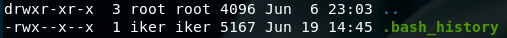
\includegraphics[scale=.75]{ls -la.png} 
\end{center}

\begin{table}[!htb]
\begin{minipage}{.5\linewidth}
      \centering
        \begin{tabular}{|c|c|}
            \hline
            Number & Permissions\\
            \hline
            0 & No permissions\\
            1 & Execute\\
            2 & Write\\
            3 & Write, Execute\\
            4 & Read\\
            5 & Read, Execute\\
            6 & Read, Write\\
            7 & Read, Write, Execute\\
            \hline
        \end{tabular}
    \end{minipage}%
    \begin{minipage}{.5\linewidth}
      \centering
        \begin{tabular}{|c|c|c|}
        	\hline
            User & Group & Others\\
            \hline
            	\begin{tabular}{ccc}-&-&-\end{tabular}&\begin{tabular}{ccc}-&-&-\end{tabular}&\begin{tabular}{ccc}-&-&-\end{tabular}\\
            	\begin{tabular}{ccc}-&-&x\end{tabular}&\begin{tabular}{ccc}-&-&x\end{tabular}&\begin{tabular}{ccc}-&-&x\end{tabular}\\
            	\begin{tabular}{ccc}-&w&-\end{tabular}&\begin{tabular}{ccc}-&w&-\end{tabular}&\begin{tabular}{ccc}-&w&-\end{tabular}\\
            	\begin{tabular}{ccc}-&w&x\end{tabular}&\begin{tabular}{ccc}-&w&x\end{tabular}&\begin{tabular}{ccc}-&w&x\end{tabular}\\
            	\begin{tabular}{ccc}r&-&-\end{tabular}&\begin{tabular}{ccc}r&-&-\end{tabular}&\begin{tabular}{ccc}r&-&-\end{tabular}\\
            	\begin{tabular}{ccc}r&-&x\end{tabular}&\begin{tabular}{ccc}r&-&x\end{tabular}&\begin{tabular}{ccc}r&-&x\end{tabular}\\
            	\begin{tabular}{ccc}r&w&-\end{tabular}&\begin{tabular}{ccc}r&w&-\end{tabular}&\begin{tabular}{ccc}r&w&-\end{tabular}\\
            	\begin{tabular}{ccc}r&w&x\end{tabular}&\begin{tabular}{ccc}r&w&x\end{tabular}&\begin{tabular}{ccc}r&w&x\end{tabular}\\
            	\hline
        \end{tabular}
    \end{minipage} 
\end{table}

\section{The System}
\subsection{Color Coded}
\begin{itemize}
\item Blue: Directory.
\item Green: Executable or recognized data file.
\item Sky Blue: Symbolic link file.
\item Yellow with black background: Device
\item Pink: Graphic image file.
\item Red: Archive file.
\item Red with black background: Broken link.
\end{itemize}

\newpage
\subsection{The Filesystem Hierarchy Standard (FHS)}
\begin{itemize}
\item \textbf{/bin}: Essential user command binaries.
\item \textbf{/etc}: Configuration files for the system.
\item \textbf{/sbin}: Essential system binaries.
\item \textbf{/usr}: Read-only user application support data \& binaries.
\begin{itemize}
\item /usr/bin: Most user commands.
\item /usr/include: Standard include files for C code.
\item /usr/lib: Obj, bin, lib files for coding and packages.
\item /usr/local: Local software (./bin ./lib ./man ./sbin ./share).
\item /usr/share: Static data shareable across all architectures.
\begin{itemize}
\item /usr/share/man: Manual pages.
\end{itemize}
\end{itemize}
\item \textbf{/var}: Variable data files.
\begin{itemize}
\item /var/cache: Application cache data.
\item /var/lib: Data modifies as programmes run.
\item /var/lock: Lock files to track resources in use.
\item /var/log: Log files.
\item /var/opt: Variable data for installed packages.
\item /var/spool: Tasks waiting to be processed:
\begin{itemize}
\item /var/spool/cron
\item /var/spool/cups
\item /var/spool/mail
\end{itemize}
\item /var/tmp: Temporary files saved between reboots.
\end{itemize}
\item \textbf{/dev}: Device files included /dev/null.
\item \textbf{/home}: User home directories.
\item \textbf{/lib}: Libraries \& kernel modules.
\item \textbf{/mnt}: Mount files for temporary filesystems.
\item \textbf{/opt}: Optional software applications.
\item \textbf{/proc}: Process \& kernel information files.
\item \textbf{/root}: Home directory for the root user.
\item \textbf{/tmp}: Is a directory used to hold temporary files. Is is a d777, so we might upload exploits to that directory, because we can execute them there.
\end{itemize}
\newpage

\section{Add users}
To add users we can use the \textbf{adduser [name]} command from the terminal. Then we can write its password. Now, if we \textbf{cat /etc/passwd}, we can see a new user. But it no longer has the password there. Password are now in the shadow file.
\begin{center}
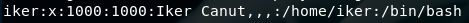
\includegraphics[scale=.75]{passwd.png} 
\end{center}

So today we have a little bit of access and information disclosure here, at hands of poor configuration. We know the name and we could use SSH and that username to try to break into the machine, but we have no hash available.\\

If we \textbf{cat /etc/shadow} we can see the passwords, hashed. Therefore, we can use a tool to break it down. It might not be easy, but there is a good chance of cracking a password.\\

If we create a new user, it will have lower priviliges. But we can change this: anybody in the sudoers file can use sudo and have root access.

\subsection{Basic Networking Commands}
Some useful basic commands:
\begin{itemize}
\item \textbf{ping}: Pinging an IP address or domain name.
\item \textbf{ifconfig}: Find interface information. Enumerates the interfaces and shows their IP Addresses, the network addresses, the broadcast addresses, packing information,... And then the Loop Back interface that's running on the system as well.
\item \textbf{ifconfig [interface] promisc}: You turn an interface into promiscuous mode. Making an interface promiscuous is essentially going to mean that is going to capture traffic it wouldn't otherwise pick up on or listen to. So it's going to pick up on everything and listen to everything. This could be good for packet captures. To turn off the promiscuous mode of an interface, just write the next command: \textbf{ifconfig [interface] -promisc}.
\item \textbf{traceroute}: Is a troubleshooting tool that can help you map out a path, see the route to a particular domain or maybe an internal system, ...
\item \textbf{netstat}: It's going to give you a slew of information about the different things that are listening and running on a system.
\item \textbf{netstat -ano}: Show the active connections that are running on your machine. You can see what's open and what's talking.
\item \textbf{nslookup}: DNS query. It shows public DNS information.
\item \textbf{dig}: Domain Information Groper. It's like nslookup but it shows more information, such us feedback from  our internal DNS server.
\item \textbf{iwconfig}: Lists wireless extensions.
\item \textbf{arp -a}: Show the IP Addresses it talks to and the MAC Addresses associated with them.
\item \textbf{route}: This will print your routing table: it tells you where your traffic exits. There could be a machine that has multiple routes, so you might see 2 different IPs because it might have a dual home NIC, so it's talking to a completely different network that you didn't know it existed.
\end{itemize}
\end{document}